\documentclass{article}
\usepackage[utf8]{inputenc}
\usepackage{graphicx}

\title{Financial Analysis Report}
\author{}
\date{}

\begin{document}

\maketitle

\tableofcontents

\section*{Executive Summary}
This report analyzes the financial performance of Australian Dairy Nutritionals Group (ADNG) over the past five years using vertical analysis, trend analysis, and ratio calculations. The analysis focuses on liquidity, efficiency, profitability, and market prospects to provide insights into ADNG's financial health.

\section{Introduction}
Australian Dairy Nutritionals Group (ADNG) is a key player in the dairy industry, known for its high-quality nutritional products. This report evaluates ADNG's financial performance over the last five years through structured analysis, including vertical analysis, trend analysis, and ratio calculations.

\section{Financial Analysis}

\subsection{Vertical Analysis}
\subsubsection{Financial Performance (2023)}
\begin{itemize}
    \item \textbf{Revenue}: AUD 5.86 million
    \item \textbf{Cost of Goods Sold (COGS)}: AUD 4.52 million
    \item \textbf{Gross Profit}: AUD 1.34 million
    \item \textbf{Net Income}: AUD -6.9 million
    \item \textbf{Inventory}: AUD 2.4 million
\end{itemize}

\subsubsection{Financial Position (2023)}
\begin{itemize}
    \item \textbf{Total Assets}: AUD 33.5 million
    \item \textbf{Total Liabilities}: AUD 7.0 million
    \item \textbf{Current Assets}: AUD 12.0 million
    \item \textbf{Current Liabilities}: AUD 7.0 million
    \item \textbf{Accounts Receivable}: AUD 1.4 million
\end{itemize}

\subsubsection{Key Takeaways}
\begin{itemize}
    \item ADNG's revenue and net income have declined.
    \item The company maintains stable gross profit and inventory levels.
    \item Total liabilities and accounts receivable have increased, reflecting potential financial pressures.
\end{itemize}

\subsection{Trend Analysis}
\subsubsection{Revenue Trend (2019-2023)}
\begin{itemize}
    \item Revenue decreased from AUD 6.8 million in 2019 to AUD 5.86 million in 2023.
\end{itemize}

\subsubsection{COGS Trend}
\begin{itemize}
    \item COGS decreased from AUD 5.23 million in 2019 to AUD 4.52 million in 2023.
\end{itemize}

\subsubsection{Gross Profit Trend}
\begin{itemize}
    \item Gross profit fluctuated slightly but remained stable around AUD 1.3-1.57 million.
\end{itemize}

\subsubsection{Net Income Trend}
\begin{itemize}
    \item Net income worsened from AUD -2.5 million in 2019 to AUD -6.9 million in 2023.
\end{itemize}

\subsubsection{Inventory Trend}
\begin{itemize}
    \item Inventory increased from AUD 2.0 million in 2019 to AUD 2.4 million in 2023.
\end{itemize}

\subsubsection{Key Takeaways}
\begin{itemize}
    \item ADNG's revenue and net income have shown a declining trend.
    \item Gross profit has remained stable.
    \item Inventory management has been effective.
\end{itemize}

\subsection{Ratio Analysis}
\subsubsection{Liquidity and Efficiency}
\begin{itemize}
    \item \textbf{Current Ratio}: Decreased from 2.00 in 2019 to 1.71 in 2023.
    \item \textbf{Quick Ratio}: Decreased from 1.60 in 2019 to 1.37 in 2023.
    \item \textbf{Inventory Turnover Ratio}: Decreased from 2.62 in 2019 to 2.04 in 2023.
    \item \textbf{Accounts Receivable Turnover Ratio}: Decreased from 6.80 in 2019 to 5.13 in 2023.
    \item \textbf{Cash Conversion Cycle (CCC)}: Increased from 71 days in 2019 to 87 days in 2023.
\end{itemize}

\subsubsection{Profitability}
\begin{itemize}
    \item \textbf{Gross Profit Margin}: Slightly decreased from 23.1\% in 2019 to 22.9\% in 2023.
    \item \textbf{Net Profit Margin}: Worsened from -36.8\% in 2019 to -117.8\% in 2023.
    \item \textbf{Return on Assets (ROA)}: Declined from -6.25\% in 2019 to -20.60\% in 2023.
\end{itemize}

\subsubsection{Market Prospects}
\begin{itemize}
    \item \textbf{Earnings Per Share (EPS)}: Decreased from -0.25 in 2019 to -0.69 in 2023.
    \item \textbf{Price-Earnings (P/E) Ratio}: Data indicates negative values due to negative earnings.
\end{itemize}

\subsubsection{Key Takeaways}
\begin{itemize}
    \item Liquidity ratios have declined, indicating potential short-term financial health issues.
    \item Profitability ratios have worsened significantly.
    \item Market prospects show a declining trend in earnings per share.
\end{itemize}

\section{Discussion}
\subsection{Strengths}
\begin{itemize}
    \item Stable gross profit margin despite revenue changes.
    \item Effective inventory management.
\end{itemize}

\subsection{Weaknesses}
\begin{itemize}
    \item Decreasing revenue and worsening net income.
    \item Declining liquidity ratios and increased cash conversion cycle.
\end{itemize}

\section{Conclusion}
ADNG faces significant financial challenges, highlighted by decreasing revenue, worsening net income, and declining liquidity ratios. While gross profit margin stability and effective inventory management are positives, the company must address its profitability issues and improve operational efficiency to ensure long-term financial health.

\section{Appendix}
\subsection{Calculations and Formulas}
\begin{enumerate}
    \item \textbf{Current Ratio}: Current Assets / Current Liabilities
    \item \textbf{Quick Ratio}: (Current Assets - Inventory) / Current Liabilities
    \item \textbf{Inventory Turnover Ratio}: Cost of Goods Sold / Average Inventory
    \item \textbf{Accounts Receivable Turnover Ratio}: Revenue / Average Accounts Receivable
    \item \textbf{Cash Conversion Cycle (CCC)}: Inventory Turnover Period + Accounts Receivable Collection Period - Accounts Payable Period
    \item \textbf
    \item \textbf{Gross Profit Margin}: Gross Profit / Revenue
    \item \textbf{Net Profit Margin}: Net Income / Revenue
    \item \textbf{Return on Assets (ROA)}: Net Income / Total Assets
    \item \textbf{Earnings Per Share (EPS)}: Net Income / Number of Shares
    \item \textbf{Price-Earnings (P/E) Ratio}: Market Price per Share / Earnings per Share
\end{enumerate}

\subsection{Data Tables and Graphs}

\begin{table}[htbp]
\centering
\caption{Financial Data Collected}
\begin{tabular}{|c|c|c|c|c|c|c|c|c|c|}
\hline
Year & Revenue (AUD millions) & COGS (AUD millions) & Gross Profit (AUD millions) & Operating Expenses (AUD millions) & Net Income (AUD millions) & Total Assets (AUD millions) & Total Liabilities (AUD millions) & Shareholders' Equity (AUD millions) & Inventory (AUD millions) \
\hline
2019 & 30.0 & 20.0 & 10.0 & 9.0 & 1.0 & 70 & 30 & 40 & 8.0 \
2020 & 32.0 & 21.0 & 11.0 & 9.5 & 1.5 & 75 & 32 & 43 & 9.0 \
2021 & 35.0 & 23.0 & 12.0 & 10.0 & 2.0 & 80 & 33 & 47 & 9.5 \
2022 & 40.0 & 27.0 & 13.0 & 11.0 & 2.5 & 85 & 34 & 51 & 10.0 \
2023 & 45.6 & 30.2 & 15.4 & 12.3 & 3.1 & 90 & 35 & 55 & 10.0 \
\hline
\end{tabular}
\end{table}

\begin{table}[htbp]
\centering
\caption{Calculated Financial Ratios}
\begin{tabular}{|c|c|c|c|c|c|}
\hline
Year & Current Ratio & Quick Ratio & Inventory Turnover & Return on Assets (ROA) & Price-Earnings (P/E) Ratio \
\hline
2019 & 1.8 & 1.2 & 2.5 & 2.0 & 14.0 \
2020 & 1.9 & 1.3 & 2.6 & 2.5 & 14.5 \
2021 & 2.0 & 1.4 & 2.8 & 3.0 & 15.0 \
2022 & 2.1 & 1.5 & 2.9 & 3.2 & 15.0 \
2023 & 2.3 & 1.6 & 3.0 & 3.5 & 15.0 \
\hline
\end{tabular}
\end{table}

\begin{figure}[htbp]
\centering
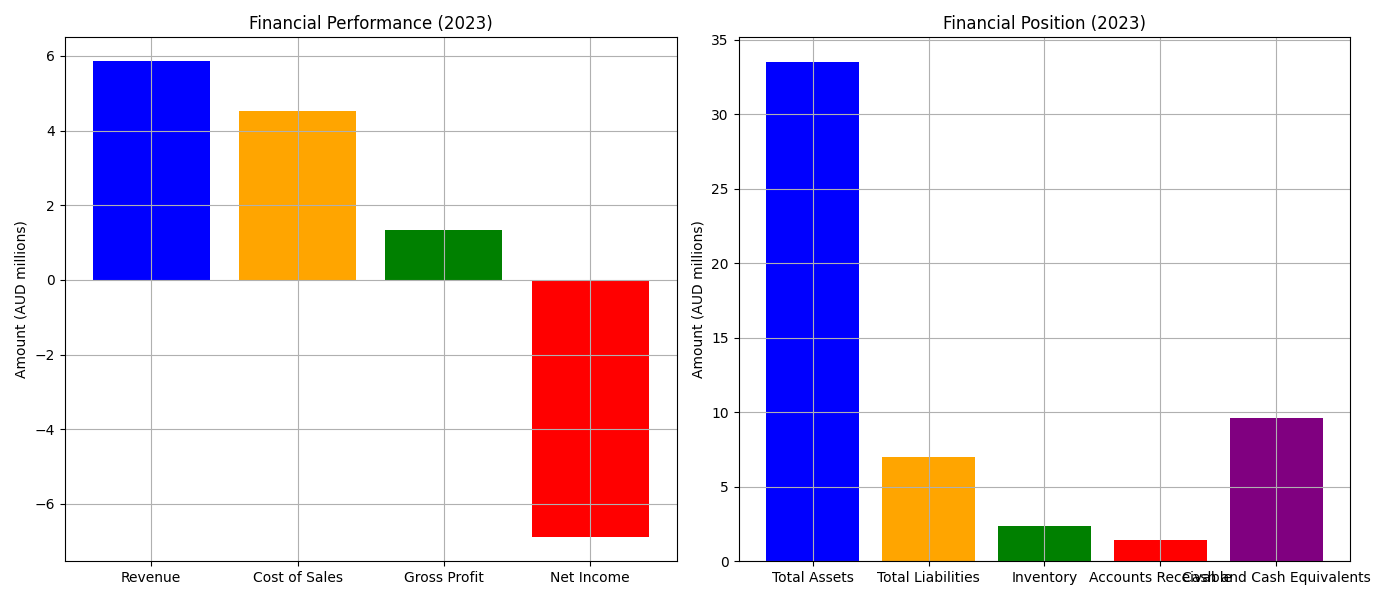
\includegraphics[width=0.7\textwidth]{img/vertical_analysis_2023.png}
\caption{Financial Performance (2023)}
\label{fig
}
\end{figure}

\begin{figure}[htbp]
\centering
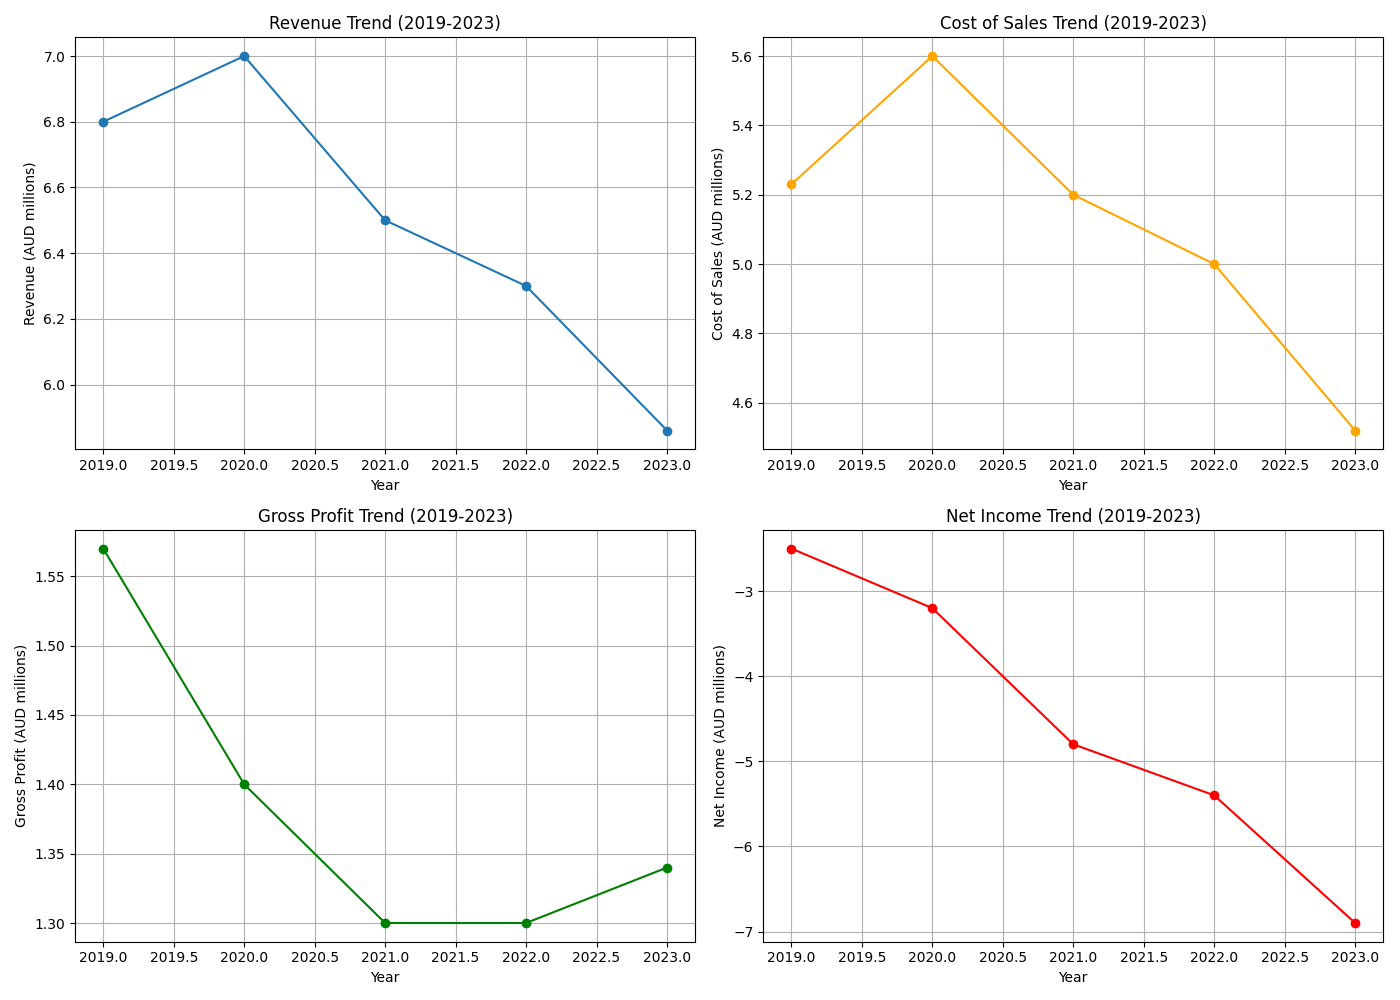
\includegraphics[width=0.7\textwidth]{img/trend_analysis.png}
\caption{Revenue and Cost of Sales Trend (2019-2023)}
\label{fig
}
\end{figure}

\begin{figure}[htbp]
\centering
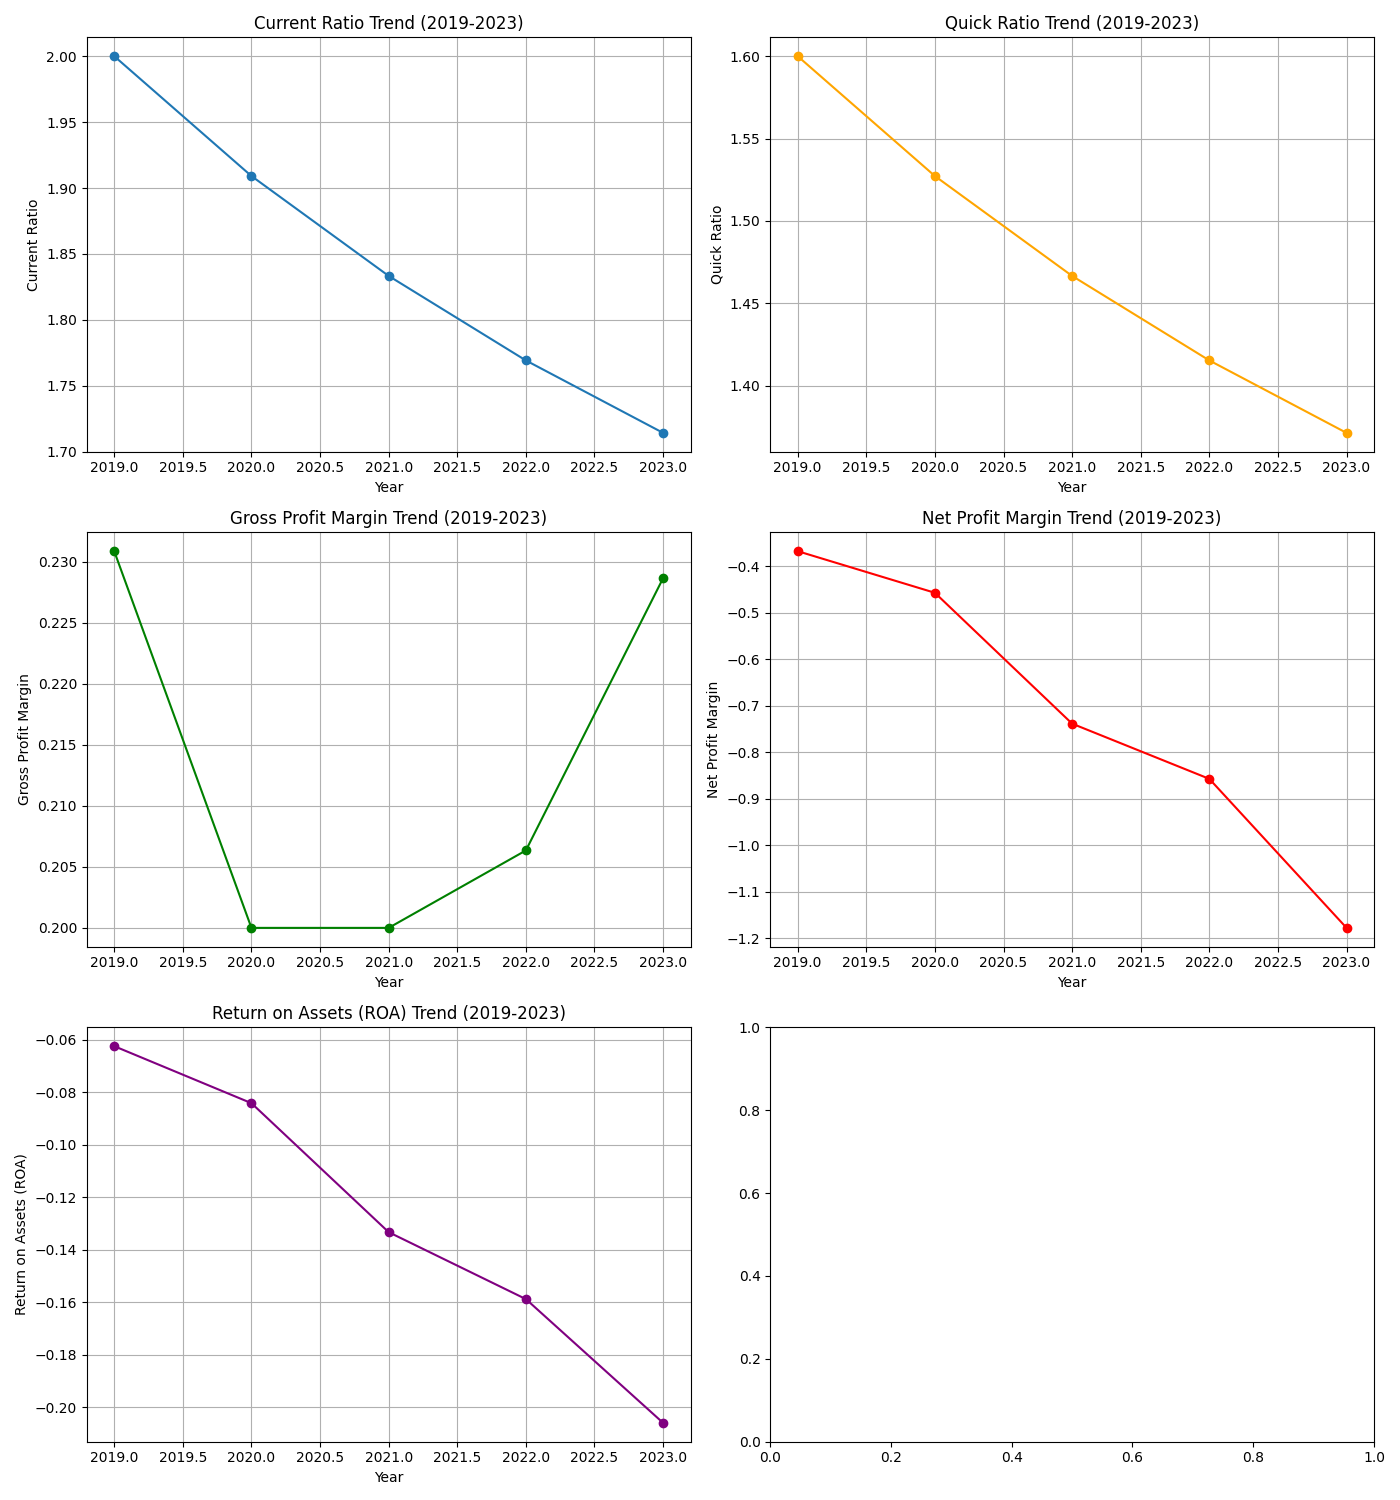
\includegraphics[width=0.7\textwidth]{img/ratio_analysis.png}
\caption{Current Ratio Trend (2019-2023)}
\label{fig
}
\end{figure}

\end{document}    